% XeLaTeX document
\documentclass[12pt,a4paper]{article}

% Редактируем: конфигурация, личные настройки: имя, название предмета и пр. для титульной страницы и метаданных документа здесь
\newcommand{\university}{Национальный исследовательский Университет ИТМО}
\newcommand{\mfaculty}{Мегафакультет информационных и трансляционных технологий}
\newcommand{\faculty}{Факультет инфокоммуникационных технологий}
\newcommand{\city}{Санкт-Петербург}
\newcommand{\num}{ №3}
\newcommand{\docname}{Лабораторная работа}
\newcommand{\subject}{Алгоритмы и структуры данных}
\newcommand{\tutorname}{В.Е. Артамонова}
\newcommand{\studentname}{И.В. Гуторова}
\newcommand{\group}{К3141}

% Не редактируем: используемые пакеты
% настройка кодировки, шрифтов и русского языка
\usepackage{fontspec}
\usepackage{polyglossia}

% рабочие ссылки в документе
\usepackage{hyperref}

% графика
\usepackage{graphicx}
\usepackage{tikz}

% поворот страницы
\usepackage{pdflscape}

% качественные листинги кода
\usepackage{minted}
\usepackage{listings}
\usepackage{lstfiracode}

% отключение копирования номеров строк из листинга, работает не во всех просмотрщиках (в Adobe Reader работает)
\usepackage{accsupp}
\newcommand\emptyaccsupp[1]{\BeginAccSupp{ActualText={}}#1\EndAccSupp{}}
\let\theHFancyVerbLine\theFancyVerbLine
\def\theFancyVerbLine{\rmfamily\tiny\emptyaccsupp{\arabic{FancyVerbLine}}}

% библиография
\bibliographystyle{templates/gost-numeric.bbx}
\usepackage{csquotes}
\usepackage[parentracker=true,backend=biber,hyperref=true,bibencoding=utf8,style=numeric-comp,language=auto,autolang=other,citestyle=gost-numeric,defernumbers=true,bibstyle=gost-numeric,sorting=ntvy]{biblatex}

% установка полей
\usepackage{geometry}

% нумерация картинок по секциям
\usepackage{chngcntr}

% дополнительные команды для таблиц
\usepackage{booktabs}

% для заголовков
\usepackage{caption}
\usepackage{titlesec}
\usepackage[dotinlabels]{titletoc}

% разное для математики
\usepackage{amsmath, amsfonts, amssymb, amsthm, mathtools}

% водяной знак на документе, см. main.tex
\usepackage[printwatermark]{xwatermark}

% Не редактируем: параметры используемых пакетов и не только
% настройки polyglossia
\setdefaultlanguage{russian}
\setotherlanguage{english}

% локализация
\addto\captionsrussian{
	\renewcommand{\figurename}{Рисунок}%
	\renewcommand{\partname}{Глава}
	\renewcommand{\contentsname}{\centerline{Содержание}}
	\renewcommand{\listingscaption}{Листинг}
}

% основной шрифт документа
\setmainfont{CMU Serif}
\newfontfamily\cyrillicfont{CMU Serif}[Script=Cyrillic]

% перечень использованных источников
\addbibresource{refs.bib}

% настройка полей
\geometry{top=2cm}
\geometry{bottom=2cm}
\geometry{left=2cm}
\geometry{right=2cm}
\geometry{bindingoffset=0cm}

% настройка ссылок и метаданных документа
\hypersetup{unicode=true,colorlinks=true,linkcolor=red,citecolor=green,filecolor=magenta,urlcolor=cyan,
	pdftitle={\docname},
	pdfauthor={\studentname},
	pdfsubject={\subject},
	pdfcreator={\studentname},
	pdfproducer={Overleaf},
	pdfkeywords={\subject}
}

% настройка подсветки кода и окружения для листингов
\usemintedstyle{colorful}
\newenvironment{code}{\captionsetup{type=listing}}{}

% шрифт для листингов с лигатурами
\setmonofont{FiraCode-Regular.otf}[
	SizeFeatures={Size=10},
	Path = templates/,
	Contextuals=Alternate
]

% оформления подписи рисунка
\captionsetup[figure]{labelsep = period}

% подпись таблицы
\DeclareCaptionFormat{hfillstart}{\hfill#1#2#3\par}
\captionsetup[table]{format=hfillstart,labelsep=newline,justification=centering,skip=-10pt,textfont=bf}

% путь к каталогу с рисунками
\graphicspath{{fig/}}

% Внесение titlepage в учёт счётчика страниц
\makeatletter
\renewenvironment{titlepage} {
	\thispagestyle{empty}
}
\makeatother

\counterwithin{figure}{section}
\counterwithin{table}{section}

\titlelabel{\thetitle.\quad}

% для удобного конспектирования математики
\mathtoolsset{showonlyrefs=true}
\theoremstyle{plain}
\newtheorem{theorem}{Теорема}[section]
\newtheorem{proposition}[theorem]{Утверждение}
\theoremstyle{definition}
\newtheorem{corollary}{Следствие}[theorem]
\newtheorem{problem}{Задача}[section]
\theoremstyle{remark}
\newtheorem*{nonum}{Решение}

% настоящее матожидание
\newcommand{\MExpect}{\mathsf{M}}

% объявили оператор!
\DeclareMathOperator{\sgn}{\mathop{sgn}}

% перенос знаков в формулах (по Львовскому)
\newcommand*{\hm}[1]{#1\nobreak\discretionary{} {\hbox{$\mathsurround=0pt #1$}}{}}


% водяной знак для обозначения статуса документа
%\newwatermark[allpages,color=red!5,angle=45,scale=3,xpos=0,ypos=0]{DRAFT}
\begin{document}
% Не редактируем: Титульная страница (формируется автоматически из заданной конфигурации)
\begin{titlepage}	% начало титульной страницы

	\begin{center}		% выравнивание по центру

		\large \university \\
		\large \mfaculty \\
		\large \faculty \\[6cm]
		% название института, затем отступ 6см

		\huge \subject \\[0.5cm] % название работы, затем отступ 0,5см
		\large \docname  \num \\[5.1cm]
		 %\large Разработка методов обучения с подкреплением\\[5cm]

	\end{center}


	\begin{flushright} % выравнивание по правому краю
		\begin{minipage}{0.25\textwidth} % врезка в половину ширины текста
			\begin{flushleft} % выровнять её содержимое по левому краю

				\large\textbf{Работу выполнил:}\\
				\large \studentname \\
				\large {Группа:} \group \\

				\large \textbf{Преподаватель:}\\
				\large \tutorname

			\end{flushleft}
		\end{minipage}
	\end{flushright}

	\vfill % заполнить всё доступное ниже пространство

	\begin{center}
		\large \city \\
		\large \the\year % вывести дату
	\end{center} % закончить выравнивание по центру

\end{titlepage} % конец титульной страницы

\vfill % заполнить всё доступное ниже пространство


% Не редактируем: Страница содержания (формируется автоматически из section, subsection и пр., указанных в content.tex)
% Содержание
\tableofcontents
\newpage



% Редактируем: всё остальное: вступление, др. этапы, заключение, приложение
\section{Задачи по варианту}

\subsection{Улучшение Quick sort}
1. Используя псевдокод процедуры Randomized - QuickSort, а так же Partition из презентации к Лекции 3 (страницы 8 и 12), напишите программу быстрой сортировки на Python и проверьте ее, создав несколько рандомных массивов, подходящих под параметры:
\begin{itemize}
	\item Формат входного файла (input.txt). В первой строке входного файла
    содержится число $n$ $(1 \le n \le 10^4)$ — число элементов в массиве.
    Во второй строке находятся n различных целых чисел, по модулю не
    превосходящих $10^9$.
	\item Формат выходного файла (output.txt). Одна строка выходного файла
    с отсортированным массивом. Между любыми двумя числами должен
    стоять ровно один пробел
	\item Ограничение по времени: 2 сек.
        \item Ограничение по памяти: 256 мб.
        \item Для проверки можно выбрать наихудший случай, когда сортируется
    массив размера $10^3$, $10^4$, $10^5$ чисел порядка $10^9$, отсортированных в обратном порядке; наилучший, когда массив уже отсортирован, и средний
    - случайный. Сравните на данных сетах Randomized-QuickSort и простой QuickSort. (А также есть Tail-Recursive-QuickSort \cite{book})

\end{itemize}

2. Основное задание. Цель задачи - переделать данную реализацию рандомизированного алгоритма быстрой сортировки, чтобы она работала быстро даже с последовательностями, содержащими много одинаковых элементов. Чтобы заставить алгоритм быстрой сортировки эффективно обрабатывать последовательности с несколькими уникальными элементами, нужно заменить двухстороннее разделение на трехстороннее \cite{alg}. То есть ваша новая процедура разделения должна разбить массив на три части:
\begin{itemize}
    \item $A[k] < x$ для всех $l + 1 \le k \le m_1 − 1$
    \item $A[k] = x$ для всех $m_1 \le  k \le m_2$
    \item $A[k] > x$ для всех $m_2 + 1 \le k \le r$
    \item Формат входного и выходного файла аналогичен п.1.
    \item Аналогично п.1 этого задания сравните Randomized-QuickSort+ c
    Partition и ее с Partition3 на сетах случайных данных, в которых
    содержатся всего несколько уникальных элементов при n = $10^3$, $10^4$, $10^5$. Что быстрее, Randomized-QuickSort+ c Partition3 или Merge-Sort?
\end{itemize}
\begin{table}[H]
    \caption{Пример}
	\begin{center}
		\begin{tabular}{|l|l|}
			\hline
			  input.txt  &  output.txt \\ \hline
			    5 2 3 9 2 2  &  2 2 2 3 9 \\ \hline
		\end{tabular}
		\label{tabular:tab_examp_2}
	\end{center}
\end{table}

\begin{code}
	\inputminted[breaklines=true, xleftmargin=1em, linenos, frame=single, framesep=10pt, fontsize=\footnotesize, firstline=1, lastline=54]{haskell}{listings/1.py}
	\caption{Код первой задачи}
\end{code}
Текстовое объяснение решения:

Импортируем модули для измерения времени и памяти, запускаем счетчик времени. Открываем файл input.txt, считываем число элементов массива, преобразовывая строку в целочисленный тип данных, считываем строку с числами, разбиваем ее по пробелам в массив. Дальше у нас описаны 6 функций. Quiksort() принимает на вход массив чисел и индексы начала и конца сортировки+1. Если индекс начала меньше индекса конца, то есть длина сортируемой части массива больше 1, то выполняется: вызываем partition(), индекс числа, с которым сравнивали все, записываем в переменную, вызываем рекурсивно функцию для части массива меньше числа и для части массива больше числа. В randomizedquicksort все аналогично, но в начале мы выбираем случайный элемент массива и меняем его местами с первым. В partition() за опорное значение принимается первый элемент массива, мы прохоrдимся по всему массиву. Если элемент меньше опорного значения, то увеличиваем счетчик таких чисел. И меняем местами этот элемент с первым, который больше опорного. В конце вне цикла меняем местами опорный элемент и последний, который меньше его. Quicksort3() и randomizedquicksort3() работают аналогично с предыдущими функциями, но принимают от partition3() два числа – индекс первого числа, который равен опорному и последнего. И сортировка происходит тогда уже только с начала до первого числа и от второго числа до конца. Partition3() высчитывает эти два числа. В целом работает аналогично partition(), но еще запоминает количество чисел равных опорному, благодаря которому считает индекс первого числа, равного опорному. Уже вне функций вызываем quicksort() для массива от начала до его длины. В дальнейшем для проведения сравнения эта строчка будет заменяться на quicksort3(), randomizedquicksort(), randomizedquicksort3(). Остальной код будет оставаться прежним.
Открываем файл output.txt для записи, записываем в него отсортированный по возрастанию массив, преобразовав в строку и удалив лишние знаки. Закрываем файлы input.txt и output.txt. Выводим в консоль время работы с начала. Подсчитываем затраты памяти и также выводим их в консоль.

Результат работы кода на примере:

\begin{figure}[H]
	\begin{center}
		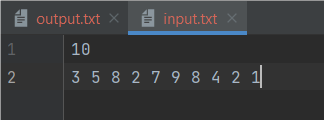
\includegraphics[scale=1]{fig/input1.png}
		\caption{Пример input файла для первой задачи}
		\label{pic:input1} % название для ссылок внутри кода
	\end{center}
        \begin{center}
		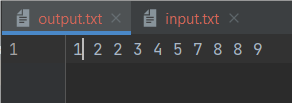
\includegraphics[scale=1.1]{fig/output1.png}
		\caption{Результат работы кода}
		\label{pic:output1} % название для ссылок внутри кода
	\end{center}
\end{figure}

Вывод по задаче:

В этой задаче мы научились сортировать массив чисел по возрастанию путем быстрой сортировки и улучшили алгоритм, а также сравнили различные варианты выполнения сортировки и сравнили с сортировкой слиянием.

\subsection{Индекс Хирша}
Для заданного массива целых чисел citations, где каждое из этих чисел – число цитирований i-ой статьи ученого-исследователя, посчитайте индекс Хирша этого ученого.

По определению Индекса Хирша на Википедии: Учёный имеет индекс h, если h из его/её Np статей цитируются как минимум h раз каждая, в то время как оставшиеся (Np − h) статей цитируются не более чем h раз каждая. Иными словами, учёный с индексом h опубликовал как минимум h статей, на каждую из которых сослались как минимум h раз.

Если существует несколько возможных значений h, в качестве h-индекса принимается максимальное из них.

\begin{itemize}
	\item Формат ввода или входного файла (input.txt). Одна строка citations, содержащая n целых чисел, по количеству статей ученого (длина citations), разделенных пробелом или запятой.

	\item Формат выхода или выходного файла (output.txt). Одно число - индекс Хирша (h-индекс).

	\item Ограничения: $1 \le n \le 5000$, 0 $\le$ citations[i] $\le$ 1000.
\end{itemize}

\begin{table}[H]
    \caption{Пример}
	\begin{center}
		\begin{tabular}{|l|l|}
			\hline
			  input.txt  &  output.txt \\ \hline
			    3,0,6,1,5  &  3 \\ \hline
		\end{tabular}
		\label{tabular:tab_examp_2}
	\end{center}
\end{table}

Пояснение. citations = [3,0,6,1,5] означает, что ученый опубликовал 5 статей в целом, и каждая из них оказалась процитирована 3, 0, 6, 1, 5 раз соответственно. Поскольку у ученого есть 3 статьи с минимум тремя цитированиями, а у оставшихся двух - не более 3 цитирований, его индекс Хирша равен 3.
\begin{table}[H]
    \caption{Пример}
	\begin{center}
		\begin{tabular}{|l|l|}
			\hline
			  input.txt  &  output.txt \\ \hline
			    1,3,1  &  1 \\ \hline
		\end{tabular}
		\label{tabular:tab_examp_2}
	\end{center}
\end{table}


\begin{itemize}
	\item Ограничений по времени (и памяти) не предусмотрено, проверьте максимальный случай при заданных ограничениях на данные, и оцените асимптотическое время.

	\item Подумайте, если бы массив citations был бы изначально отсортирован по возрастанию, можно было бы еще ускорить алгоритм?

\end{itemize}

\begin{code}
	\inputminted[breaklines=true, xleftmargin=1em, linenos, frame=single, framesep=10pt, fontsize=\footnotesize, firstline=1, lastline=38]{haskell}{listings/12.py}
	\caption{Код второй задачи}
\end{code}
Текстовое объяснение решения:

Импортируем модули для измерения времени и памяти, запускаем счетчик времени. Открываем файл input.txt, считываем число элементов массива, преобразовывая строку в целочисленный тип данных, считываем строку с числами, разбиваем ее по запятым в массив. Используем функции из первой задачи, чтобы отсортировать массив. Также немного изменим potition(). Теперь она будет принимать  на вход еще и опорный элемент. Сортируем массив. Создаем переменную для индекса, изначально равную 0. В цикле проходим по всем числам от 0 до максимального в массиве. Вызываем partition() для этого числа, таким образом находим индекс первого числа, большего рассматриваемого. Если количество чисел, которые больше данного числа, больше данного числа, приравниваем индекс Хирша к нему. Если нет, выходим из цикла, дальше ничего быть не может.Открываем файл output.txt для записи, записываем в него индекс Хирша. Закрываем файлы input.txt и output.txt. Выводим в консоль время работы с начала. Подсчитываем затраты памяти и также выводим их в консоль.

Результат работы кода на примере:

\begin{figure}[H]
	\begin{center}
		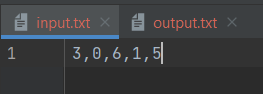
\includegraphics[scale=1.1]{fig/input12.png}
		\caption{Пример input файла}
		\label{pic:input12} % название для ссылок внутри кода
	\end{center}
        \begin{center}
		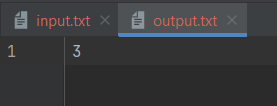
\includegraphics[scale=1]{fig/output12.png}
		\caption{Результат работы кода}
		\label{pic:output12} % название для ссылок внутри кода
	\end{center}
\end{figure}

Вывод по задаче:

В этой задаче мы научились высчитывать индекс Хирша и применили быструю сортировку на практике.
 
\section{Дополнительные задачи}

\subsection{Сортировка пугалом}
«Сортировка пугалом» — это давно забытая народная потешка. Участнику
под верхнюю одежду продевают деревянную палку, так что у него оказываются растопырены руки, как у огородного пугала. Перед ним ставятся n матрёшек в ряд. Из-за палки единственное, что он может сделать — это взять в руки две матрешки на расстоянии k друг от друга (то есть i-ую и i + k-ую), развернуться и поставить их обратно в ряд, таким образом поменяв их местами.
Задача участника — расположить матрёшки по неубыванию размера. Может ли он это сделать?

\begin{itemize}
	\item Формат входного файла (input.txt). В первой строчке содержатся числа n и k $(1 \le n, k \le 10^5)$ – число матрёшек и размах рук. Во второй строчке содержится n целых чисел, которые по модулю не превосходят $10^9$ – размеры матрёшек.
	\item Формат выходного файла (output.txt). Выведите «ДА», если возможно отсортировать матрёшки по неубыванию размера, и «НЕТ» в противном случае.
	\item Ограничение по времени: 2 сек.
        \item Ограничение по памяти: 256 мб.

\end{itemize}

\begin{table}[H]
    \caption{Пример}
	\begin{center}
		\begin{tabular}{|c|c|}
			\hline
			  input.txt  &  output.txt \\ \hline
			    3 2 2 1 3  & НЕТ \\ \hline
                5 3 1 5 3 4 1  & ДА \\ \hline
		\end{tabular}
		\label{tabular:tab_examp_2}
	\end{center}
\end{table}

\begin{code}
	\inputminted[breaklines=true, xleftmargin=1em, linenos, frame=single, framesep=10pt, fontsize=\footnotesize, firstline=1, lastline=35]{haskell}{listings/2.py}
	\caption{Код первой дополнительной задачи}
\end{code}
Текстовое объяснение решения:

Функция выполняет сортировку пугалом: в цикле проходим по каждому элементу массива до n-k. Сравниваем текущий элемент и элемент, который на k впереди. Если первый больше, меняем их местами.
Запускаем счетчик времени. Открываем файл input.txt, считываем входные данные. Открываем файл output.txt для записи. Вызываем функцию сортировки. Создаем переменную для результата со значением «да». В цикле проходим по каждому элементу отсортированного массива, если элемент больше следующего, присваиваем переменной значение «нет». Записываем в output.txt результат. Закрываем файлы input.txt и output.txt. 

Результат работы кода на примере:

\begin{figure}[H]
	\begin{center}
		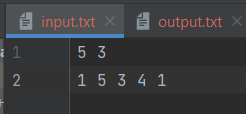
\includegraphics[scale=1]{fig/input2.png}
		\caption{Пример input файла}
		\label{pic:input2} % название для ссылок внутри кода
	\end{center}
        \begin{center}
		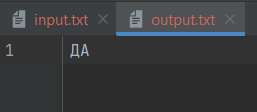
\includegraphics[scale=0.9]{fig/output2.png}
		\caption{Результат работы кода}
		\label{pic:output2} % название для ссылок внутри кода
	\end{center}
\end{figure}

Вывод по задаче:

В этой задаче мы осуществлять сортировку пугалом и определять, когда она работает.

\newpage
\section*{Вывод}
В этой лабораторной работе мы изучили способы быстрой сортировки и сортировку пугалом. Также решили прикладную задачу - расчет индекса Хирша.
\addcontentsline{toc}{section}{Вывод}

% Не редактируем: Страница библиографии (формируется автоматически из книжек, указанных в refs.bib и пометок \cite{имя_источника} в тексте)
\newpage
\printbibliography[title=Список использованных источников]
\addcontentsline{toc}{section}{Список использованных источников}
\end{document}
